\documentclass[11pt]{article}
\usepackage[english]{babel}
\usepackage[utf8]{inputenc}
\usepackage{fancyhdr}
\usepackage{graphicx}

\def\Name{Ran Liao}
\def\Topic{Software Process}

\title{\textbf{\Topic}}
\author{\Name}
\markboth{Notes on \Topic\ }{Notes on \Topic\ }
\date{\today}
 
\pagestyle{fancy}
\fancyhf{}
\rhead{\date{\today} }
\lhead{Notes on \Topic\ }
\rfoot{\thepage}

\textheight=9in
%\textwidth=6.5in
\topmargin=-.75in
%\oddsidemargin=0in
%\evensidemargin=0in
 
\begin{document}
\maketitle
\noindent\makebox[\linewidth]{\rule[8pt]{5in}{0.5pt}}

\section*{Workflow}

\begin{enumerate}
	\item \textbf{Requirements Workflow}
	
	Determine the client’s needs.
	
	The requirements artifacts must be totally comprehensible by the client. Therefore, the artifacts of the requirements workflow must therefore be expressed in a natural (human) language. However, all natural languages are imprecise.
	
	\item \textbf{Analysis Workflow}
	
	Analyze and refine the requirements. 
	
	The analysis artifacts must be precise, and complete enough for the designers.
	
	\item \textbf{Design Workflow}
	
	Refine the analysis workflow until the material is in a form that can be implemented by the programmers.
	
	Many nonfunctional requirements need to be finalized at this time, including
	
	\begin{itemize}
		\item  Choice of programming language
		\item Reuse issues
		\item Portability issues
	\end{itemize}
	
	\item \textbf{Implementation Workflow}
	
	Implement the target software product in the selected implementation language.
	
	\item \textbf{Test Workflow}
	
	The test workflow is the responsibility of every developer and maintainer, and the quality assurance group.
	
\end{enumerate}'

\section*{Phase}

\begin{enumerate}

	\item \textbf{Inception Phase}
	
	Determine whether the proposed software product is economically viable.
	
	\item \textbf{Elaboration Phase}
	
	Refine the initial requirements.
	
	\item \textbf{Construction Phase}
	
	Produce the first operational-quality version of the software product. This is sometimes called the beta release.
	
	\item \textbf{Transition Phase}
	
	Ensure that the client’s requirements have indeed been met.
	
\end{enumerate}


\section*{Unified Process}

The Unified Process is an adaptable methodology and a modeling technique. Every step performed in the Unified Process falls into one of the five core workflows and also one of the four phases. Workflow represents the technical context of a step, whereas phase represents the business context of a step.

\begin{figure}[h]
	\centering
	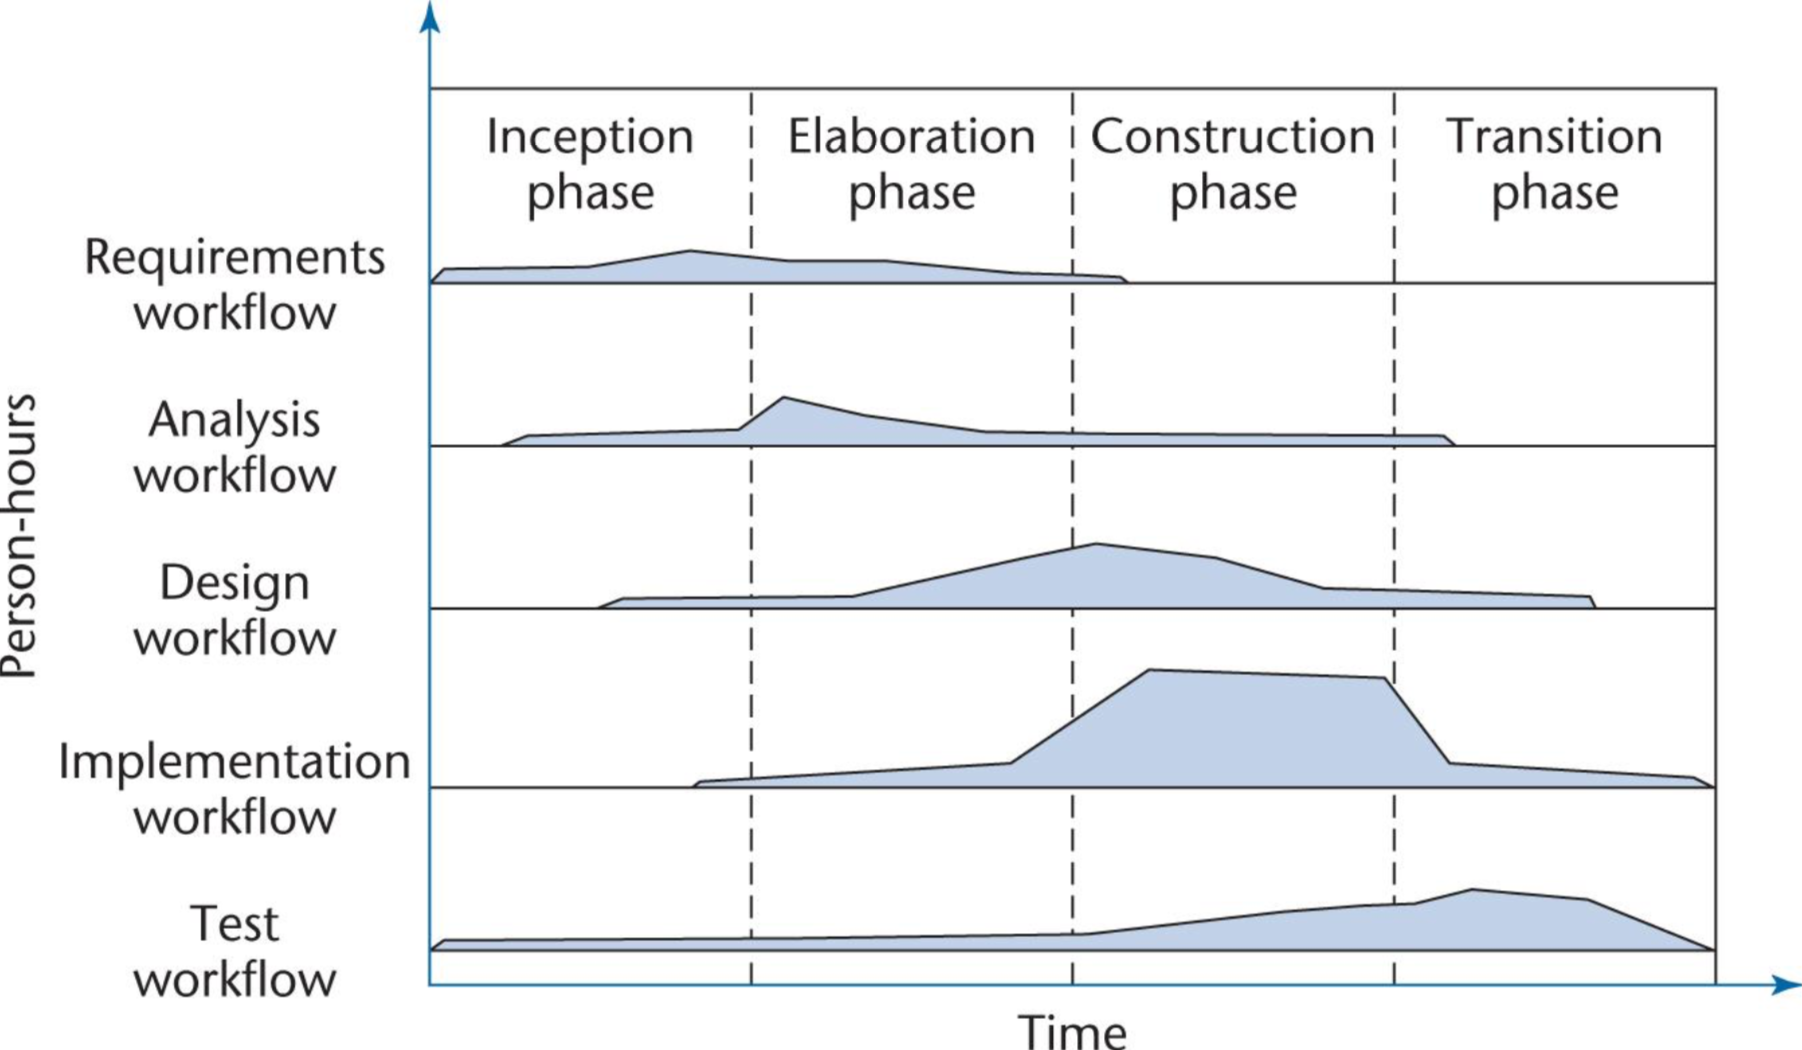
\includegraphics[width=0.9\linewidth]{images/UnifiedProcess.png}
	\caption{The Phases of the Unified Process}
	\label{fig:UnifiedProcess}
\end{figure}




\end{document}